\subsection[Image Segmentation]{Image Segmentation}
%\begin{frame}
%
%	\frametitle{Il Clustering nella segmentazione delle immagini}
%
%	\begin{block}{Clustering}
%		Come già detto lo scopo del clustering è rilevare i gruppi naturali (cluster) nei dati:
%
%		\begin{itemize}
%			\item naturale significa che i gruppi dovrebbero corrispondere a qualche interpretazione umana
%			\item ogni cluster deve essere composto da punti per i quali la similarità agli altri punti all'interno di dello stesso cluster è superiore alla similarità rispetto a punti appartenenti ad altri clusters
%			\item questo pone il problema di come misurare la similarità tra punti e, eventualmente, tra cluster
%			\item diverse misure di similarità producono differenti risultati di clusterizzazione
%		\end{itemize}
%	\end{block}
%
%\end{frame}


\begin{frame}

	\frametitle{Il clustering: segmentazione delle immagini}

%	\begin{block}{}
		Come detto, una delle applicazioni più comuni del clustering è la \textbf{segmentazione delle immagini}.
		\newlinedouble
		Questo ambito ci aiuterà molto soprattutto per facilitare la trattazione delle varie tecniche e poter avere un riscontro/confronto visivo diretto tra le varie tecniche di clusterizazzione.
		\begin{itemize}
			\item una volta completato il clustering, ogni cluster viene associato con una label (o un ID) e la posizione del centro del cluster nello spazio delle caratteristiche
			\item la segmentazione dell'immagine si ottiene associando ad ogni pixel dell'immagine l'etichetta (o il centro) del cluster a cui appartiene nello spazio delle features
			\item sono state proposte diverse tecniche di clustering. Dato un dataset, diverse tecniche di clustering possono produrre risultati differenti
		\end{itemize}
%	\end{block}

\end{frame}


\begin{frame}

	\frametitle{Il clustering: segmentazione delle immagini}

%	\begin{block}{}

		\begin{columns}

			\column{0.5\linewidth}
			\begin{itemize}
				\item si noti che un cluster non corrisponde necessariamente a una regione dell'immagine
				\item una regione percettivamente saliente può essere costituita da più cluster o più regioni
				\ifthenelse{\boolean{highschool}}{}{
					\item potrebbe essere necessario decidere qual è il migliore
					\item a tal fine è necessaria una certa misura della qualità del clustering
				}
			\end{itemize}

			\column{0.5\linewidth}
			\begin{figure}[!htbp]
				\centering
				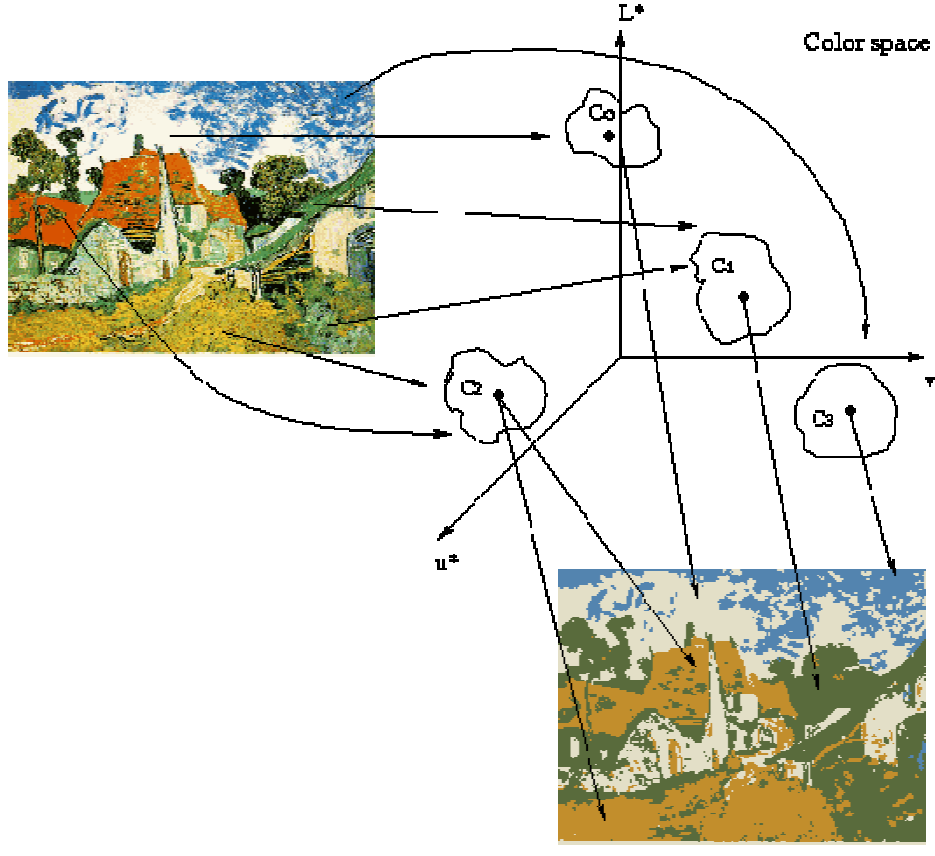
\includegraphics[width=6.0cm]{images/unsupervised/image_segmentation/image_segmentation.png}
				%\caption{ENEL QQ-Plot Normale}
				%\label{Enel_QQ_Plot_Normal}
			\end{figure}

		\end{columns}

%	\end{block}

\end{frame}


\ifthenelse{\boolean{highschool}}{}{
	\begin{frame}
	
		\frametitle{Il clustering: segmentazione delle immagini}
	
		%	\begin{block}{}
	
				Una \textbf{misura quantitativa della qualità dei risultati} del clustering è la distanza media dei punti del cluster dal loro centro del cluster.
	
				\begin{empheq}[box=\fcolorbox{blue!40!black!60}{yellow!10}]{align*}
					\mathbf{J} = \frac{1}{N} \sum_{i=1}^{N}\sum_{k=1}^{K}r_{ik} \Vert x_i-\mu_k\Vert^2
				\end{empheq}
				Dove:
				\begin{itemize}
					\item $x_i\text{ }i=1,...,N$ i punti del dataset (data point)
					\item $\mu_k\text{ }k=1,...,K$ i centri dei clusters
					\item $r_{ik}$ un indicatore binario che vale:
					\begin{itemize}
						\item[--] 1 se il punto $x_i$ appartiene al cluster $k$ con centro $\mu_k$
						\item[--] 0 altrimenti
					\end{itemize}
				\end{itemize}
		%	\end{block}
	
	\end{frame}
	
	
	\begin{frame}
	
		\frametitle{Il clustering: segmentazione delle immagini}
	
		%	\begin{block}{}
				\begin{empheq}[box=\fcolorbox{blue!40!black!60}{yellow!10}]{align*}
					\mathbf{J} = \frac{1}{N} \sum_{i=1}^{N}\sum_{k=1}^{K}r_{ik} \Vert x_i-\mu_k\Vert^2
				\end{empheq}
				Va osservato che il valore di $\mathbf{J}$ può essere utilizzato per confrontare i risultati del clustering a condizione che il numero di cluster $K$ sia lo stesso:
				\begin{itemize}
					\item il valore di $\mathbf{J}$ non può essere utilizzato per confrontare due risultati di clustering se sono stati costruiti con un numero di clusters $K$ diverso
				\end{itemize}
				Infatti, se il valore di $K$ non fosse vincolato, il clustering ottimale risulterebbe nella soluzione banale:
				\begin{itemize}
					\item ogni punto del dataset definisce un cluster, $K = N$, $J = 0$
				\end{itemize}
		%	\end{block}
	
	\end{frame}
	
	\begin{frame}
	
		\frametitle{Il clustering: segmentazione delle immagini}
	
		%	\begin{block}{}
			La scelta del numero dei cluster $K$ è un problema impegnativo.\\
			La scelta ottimale di $K$ dovrebbe essere un compromesso tra:
			\begin{itemize}
				\item la massima compressione dei dati, ottenuta utilizzando un singolo cluster
				\item la massima accuratezza ottenuta definendo un cluster per ogni data point
			\end{itemize}
			Quando il numero di cluster $K$ non è noto in anticipo, è necessario considerare alcune misure della qualità del clustering per diversi valori $K$ e si seleziona il valore di $K$ per massimizzare questa misura di qualità
		%	\end{block}
	
	\end{frame}
}
